\documentclass{article}

\usepackage{graphicx}
\usepackage{tikz}
\usepackage{tikzsymbols}
\usetikzlibrary{calc,patterns,shapes.geometric}
\pagestyle{empty}
\usepackage[margin=0pt]{geometry}
\geometry{papersize={14in,12in}}

\def\centerarc[#1](#2)(#3:#4:#5){\draw[#1] ($(#2)+({#5*cos(#3)},{#5*sin(#3)})$) arc (#3:#4:#5);}

\begin{document}
	\begin{figure}
		\centering
		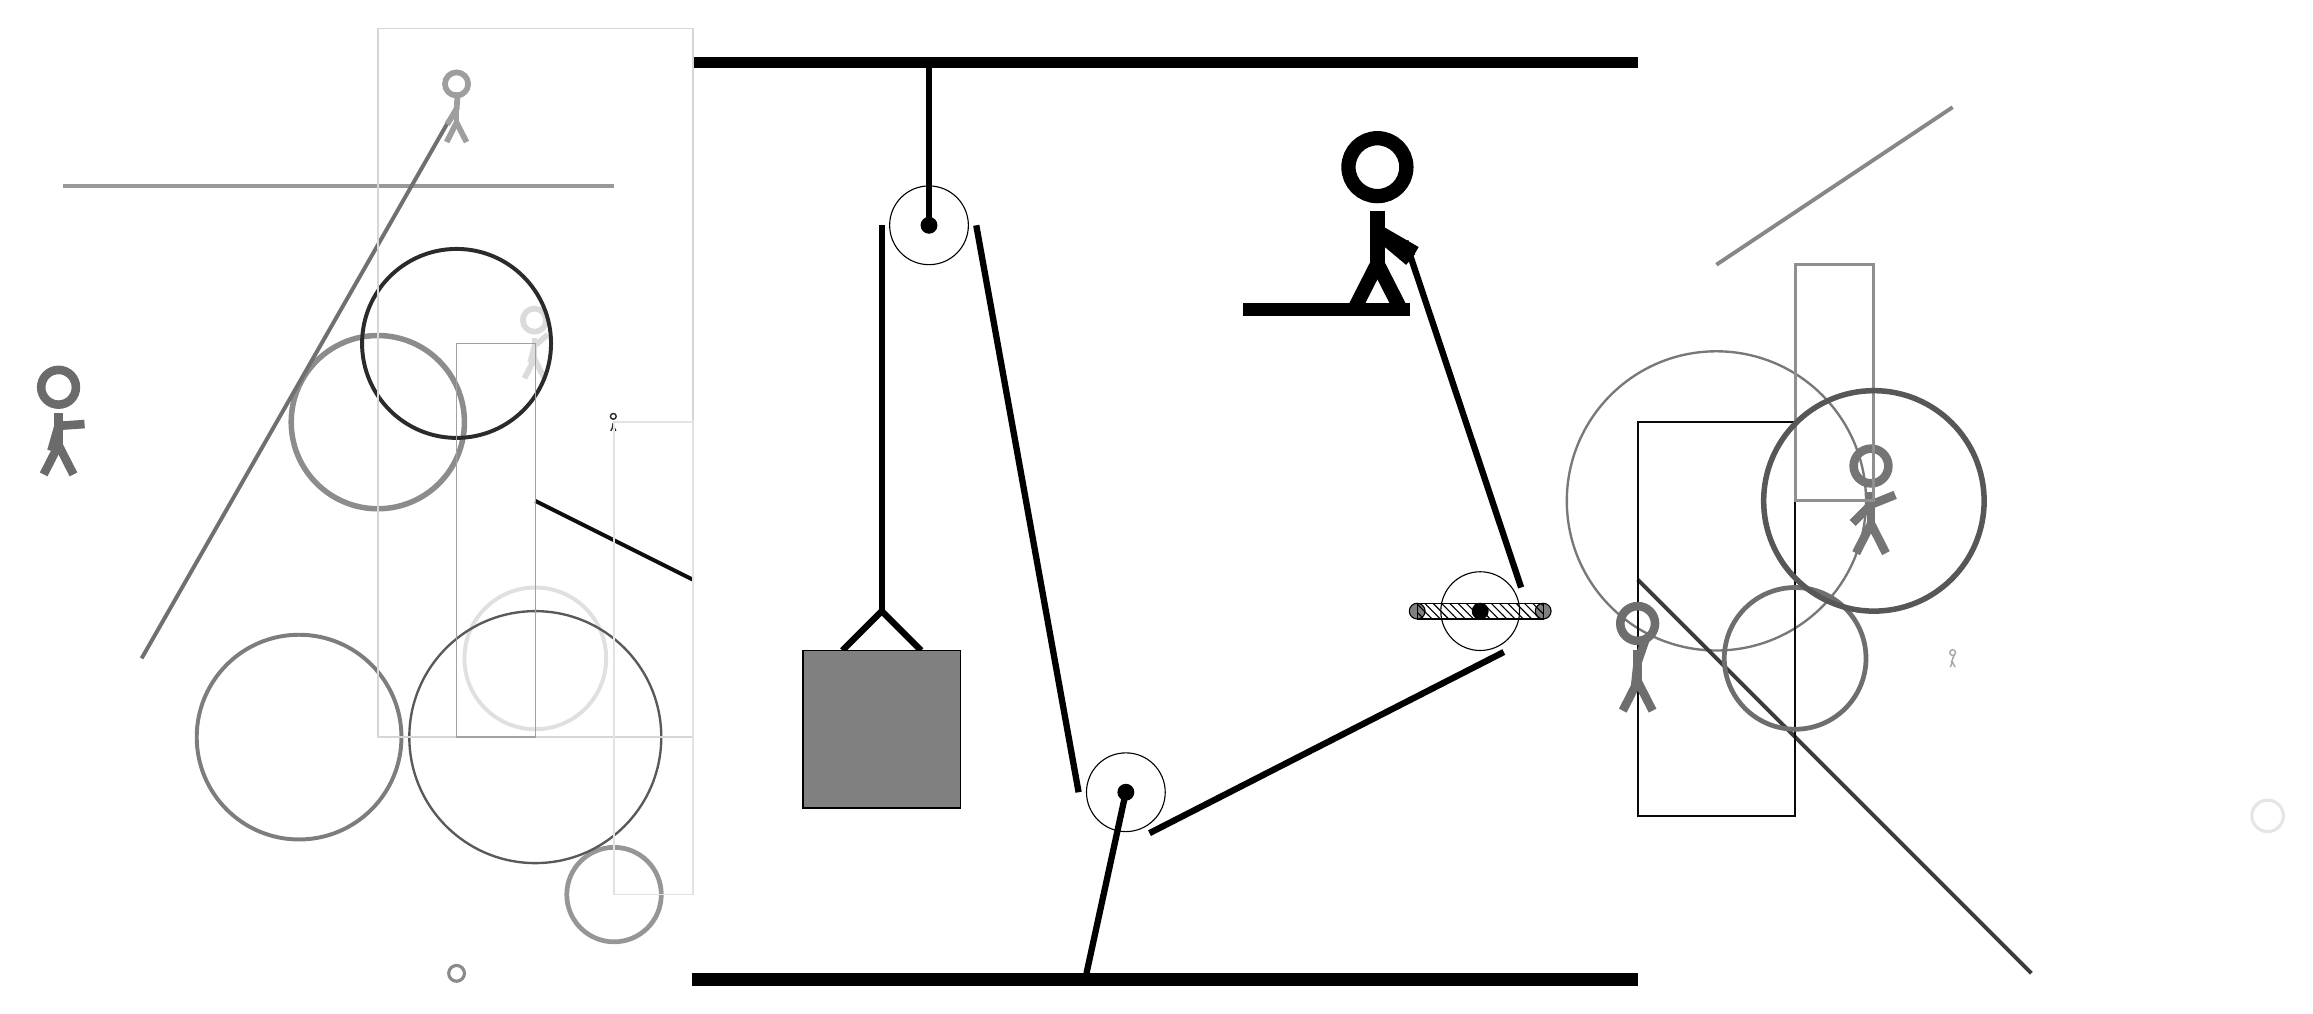
\begin{tikzpicture}
			%%%%% START %%%%%
			
			\draw[fill=black] (-2, 11.5) rectangle (10, 11.625);
			
			\draw (1, 9.5) circle (0.5);
			\draw[fill=black] (1, 9.5) circle (0.1);
			\draw[line width=0.8mm] (1, 11.5) -- (1, 9.5);
			
			\node[line width=0.2mm, color=black!14] at (-4, 8) {\Strichmaxerl[4][76][40]};
			
			\node[line width=0.7mm, color=black!58] at (-10, 7) {\Strichmaxerl[6][74][4]};
			\draw[line width=0.5mm, color=black!40](-3, 10) -- (-10, 10);
			\draw [line width=0.6mm, color=black!41](-3, 1) circle (0.6);
			\draw [line width=0.3mm, color=black!53](11, 6) circle (1.9);
			\draw[line width=0.5mm, color=black!77](10, 5) -- (15, 0);
			\draw [line width=0.5mm, color=black!51](-7, 3) circle (1.3);
			\node[line width=0.5mm, color=black!83] at (-3, 7) {\Strichmaxerl[1][78][0]};
			\node[line width=0.7mm, color=black!54] at (13, 6) {\Strichmaxerl[6][45][22]};
			\draw [line width=0.7mm, color=black!45](-6, 7) circle (1.1);
			\draw [line width=0.5mm, color=black!83](-5, 8) circle (1.2);
			
			\draw[line width=0.3mm, color=black!96] (12, 7) rectangle (10, 2);
			\draw[line width=0.5mm, color=black!47](11, 9) -- (14, 11);
			
			\draw[line width=0.5mm, color=black!56](-5, 11) -- (-9, 4);
			\node[line width=0.4mm, color=black!57] at (10, 4) {\Strichmaxerl[6][84][71]};
			\draw[line width=0.4mm, color=black!44] (12, 6) rectangle (13, 9);
			
			\draw [line width=0.6mm, color=black!57](12, 4) circle (0.9);
			\draw [line width=0.7mm, color=black!66](13, 6) circle (1.4);
			\node[line width=0.3mm, color=black!38] at (-5, 11) {\Strichmaxerl[4][57][86]};
			\draw [line width=0.4mm, color=black!46](-5, 0) circle (0.1);
			\node[line width=0.2mm, color=black!34] at (14, 4) {\Strichmaxerl[1][70][67]};
			
			\draw [line width=0.4mm, color=black!10](18, 2) circle (0.2);
			\draw [line width=0.5mm, color=black!12](-4, 4) circle (0.9);
			\draw [line width=0.3mm, color=black!65](-4, 3) circle (1.6);
			\draw[line width=0.2mm, color=black!16] (-2, 12) rectangle (-6, 3);
			
			\draw[line width=0.5mm, color=black!95](-4, 6) -- (-2, 5);
			\draw[line width=0.2mm, color=black!37] (-4, 3) rectangle (-5, 8);
			\draw[line width=0.2mm, color=black!11] (-3, 7) rectangle (-2, 1);
			
			
			\draw (3.5, 2.3) circle (0.5);
			\draw[fill=black] (3.5, 2.3) circle (0.1);
			\draw[line width=0.8mm] (3.5, 2.3) -- (3.0, 0);
			
			\draw[fill=white](8, 4.6) circle (0.5);
			\draw[fill=black] (8, 4.6) circle (0.1);
			\draw[fill=black!50] (8.8, 4.6) circle (0.1);
			\draw[fill=black!50] (7.2, 4.6) circle (0.1);
			\draw[pattern=north west lines, pattern color=black] (7.2, 4.7) rectangle (8.8, 4.5);
			
			\draw[line width=0.8mm](-0.1, 4.1) --  (0.4, 4.6) -- (0.9, 4.1);
			\draw[fill=black!50] (-0.6, 4.1) rectangle (1.4, 2.1);
			
			\draw[line width=0.8mm](0.4, 9.5) -- (0.4, 4.6);
			\centerarc[line width=0.8mm](1, 9.5)(180:0:0.6)
			\draw[line width=0.8mm](1.6, 9.5) -- (2.9, 2.3);
			\centerarc[line width=0.8mm](3.5, 2.3)(180:300:0.6);
			\draw[line width=0.8mm](3.8, 1.7804) -- (8.3, 4.0804);
			\centerarc[line width=0.8mm](8, 4.6)(300:390:0.6);
			\draw[line width=0.8mm](8.5196, 4.9) -- (7.05, 9.3);
			
			\node at (6.75, 9.5) {\Strichmaxerl[10][-220][-30]};
			\draw[fill=black] (5, 8.5) rectangle (7.1, 8.35);
			
			\draw[fill=black] (-2, 0) rectangle (10, -0.15);
			
			%%%%% END %%%%%
		\end{tikzpicture}
	\end{figure}	
\end{document}